\documentclass[12pt]{article}
\usepackage[english]{babel}
\usepackage{graphicx, amsmath, amsfonts, amsthm, mathtools, listings, color, caption, rotating, subfigure, fullpage, textcomp, enumerate, float, listings, MnSymbol, wasysym}

\lstset{
	language=R,
	keywordstyle=\bfseries\ttfamily\color[rgb]{0,0,1},
	identifierstyle=\ttfamily,
	commentstyle=\color[rgb]{0.133,0.545,0.133},
	stringstyle=\ttfamily\color[rgb]{0.627,0.126,0.941},
	showstringspaces=false,
	basicstyle=\tiny,
	numberstyle=\scriptsize,
	numbers=left,
	stepnumber=1,
	numbersep=10pt,
	tabsize=2,
	breaklines=true,
	breakatwhitespace=false,
	aboveskip={1.5\baselineskip},
  columns=fixed,
  upquote=true,
  extendedchars=true,
}

\begin{document}
\begin{center}
STA250, Homework 4 \\
Christopher Aden\\
December 7, 2013\
\end{center}

\section{Generating Truncated Normals on the GPU}
The objective of this section to sample from a truncated normal distribution on the GPU. This is necessary in some survival models, and, as we'll see later, probit regression. A random variable $X$ having a truncated normal distribution with mean $\mu$ and standard deviation $\sigma$ and truncation points $(a,b)$ can be thought of as a $N(\mu, \sigma^2)$, with support defined instead on $(a,b)$, and re-normalized to make it a valid PDF.

Sampling is accomplished several ways, each with pros and cons. I will detail all the implementations I use in my code. To ease notation, let $a' = (a-\mu)/\sigma$ and similar for $b'$. This will allow us to work on standard normals and rescale at the end.
\begin{enumerate}[A.]
\item Inverse-CDF:
	\begin{itemize}
	\item Draw $u \sim U[\Phi(a'), \Phi(b')]$.
	\item Compute $z = \Phi^{-1}(u)$.
	\item $x = \sigma * z + \mu \sim TN(\mu, \sigma^2, (a,b))$.
	\end{itemize}
\item Naive Rejection Sampling
	\begin{itemize}
	\item Draw $x \sim N(\mu, \sigma)$
	\item If $x \in (a,b)$, return $x$. Else, repeat.	
	\end{itemize}
\item One-Sided Truncation using Truncated Exponential
	\begin{itemize}
	\item Require either $a = -\infty$ or $b  = \infty$. Call $T = a'$ if $b=\infty$, or $T=-b'$ if $a=\infty$.
	\item Draw $z \sim Exp(\alpha) + T$, a truncated exponential, where $\alpha = \frac{T + \sqrt{T^2 + 4}}{2}$.
	\item If $T < \alpha$, let $\log \rho = - (z-\alpha)^2 /2$ Else, $\log \rho = \frac{(T-\alpha)^2 - (\alpha -z)^2}{2}$.
	\item Draw $u \sim U(0,1)$. If $\log{u} \leq \log \rho$ and $T=a'$, return $x = \mu + \sigma * z$. Else if $\log{u} < \log \rho$ and $T=-b'$, return $x = -\mu + \sigma * z$. Else, repeat.
	\end{itemize}
\item Robert (2009) Rejection Sampling
	\begin{itemize}
	\item Draw $z \sim U(a', b')$, $u \sim U(0,1)$.
	\item If $a' < 0$ and $b' > 0$, let $\log \rho = -z^2 /2$. Else if $a' > 0$, $\log \rho = - ({a'}^2 - z^2) /2$. Else, $\log \rho = - ({b'}^2 - z^2) /2$.
	\item If $\log u \leq \log \rho$, return $x = \mu + \sigma * z$. Else, repeat.
	\end{itemize}
\end{enumerate}

The inverse-CDF method is extremely fast and returns samples every single time. This means there is no looping and no throwing away samples. It, however, has very poor behavior when the truncation region is very far away from the mean, because of difficulty in calculating the CDF and inverse-CDF in single-precision floating point math. Through heuristics, I found this method unstable when the closest truncation point point was more than four standard deviations away from the mean. Luckily, that means this method is appropriate the vast majority of the time.

The Naive rejection sampling scheme was easy to write, but suffers a similar problem as the inverse-CDF method. It is numerically more stable for extreme truncation, but what it has in numerical stability it makes an unbelievable sacrifice in speed for. This method only exists as a fallback for inverse-CDF. I was more willing to make a sacrifice in stability in exchange for speed, as we would expect a $N(0,1, (1.645, \infty))$ to require 20 repetitions before getting even one value!

The one-sided truncation method is extremely effective and is able to beat the two naive methods in both speed and precision handily, provided there is only one point of truncation. Logarithms were used to make it more stable in the tails, and theoretical results show that as the truncation point approaches the unbounded side of the support, our acceptance probability goes to 1. This makes for efficient sampling in the tails.

The two-sided method proposed by Christian Robert is slower than the one-sided method in many cases, but is still more effective than the naive rejection sampling algorithm unless the truncation points are close to the mean. For this reason, we use it when we have two-sided truncation in the tails to similar success as the previous method.

Implementing this on the GPU was a near-triviality, given the embarrassingly parallel nature of the task. In the interest of not blowing my stack, arguments could be passed in as much smaller arrays than the total number of samples, and their arguments were recycled. This means I only needed one really large memory copy--the one from the device to the host with all the samples.

Confirming the behavior of the sampler, the sample mean of 10,000 samples was not super close to the mean (sample mean: $0.962903$. True Mean: $0.957007$), but the approximation did get better with more samples. There is also the added handicap of the GPU using single-precision floating point numbers. The CPU implementation was able to get much closer (sample mean: $0.959399$, true mean: $0.957007$).

An implementation in the \verb+msm+ package written mostly in serial C was still drastically faster than my CUDA implementation for sampling from $TN(2,1, (0, 1.5))$.
\begin{figure}[H] \center
\includegraphics[scale=.60]{TruncNorm/TruncNorm_Timings}
\end{figure}
There are likely a few factors at play here. The algorithms were just fine--I originally wrote my GPU code entirely in C (including the memory management) and the speed was fantastic. Using RCUDA, I imported the kernel's LLVM code, specified the number of blocks and grids, copied the parameters to the device, then let R run the kernel. Perhaps it was my initialization of the results vector. I'm about 90\% sure the reason the GPU code was much slower was inappropriate allocation of the device and host memory, and incorrect copies. Smarter programming could've drastically brought the run time down, since the GPU handles the computation drastically faster than the serial CPU implementation. I was unable to generate 100,000,000 truncated normal samples using either GPU or CPU, as R was unable to hold them in memory, and CUDA couldn't allocate an array that large. Potentially, I could've run the code to the maximum amount of usable memory, then stored the results on disk until they were needed.

At least it managed to correctly sample from $TN(2,1,(-\infty, \infty))$ and $TN(0, 1, (-\infty, -10))$, so while it's slow, at least it gets the answers right.
\begin{figure}[H] \center
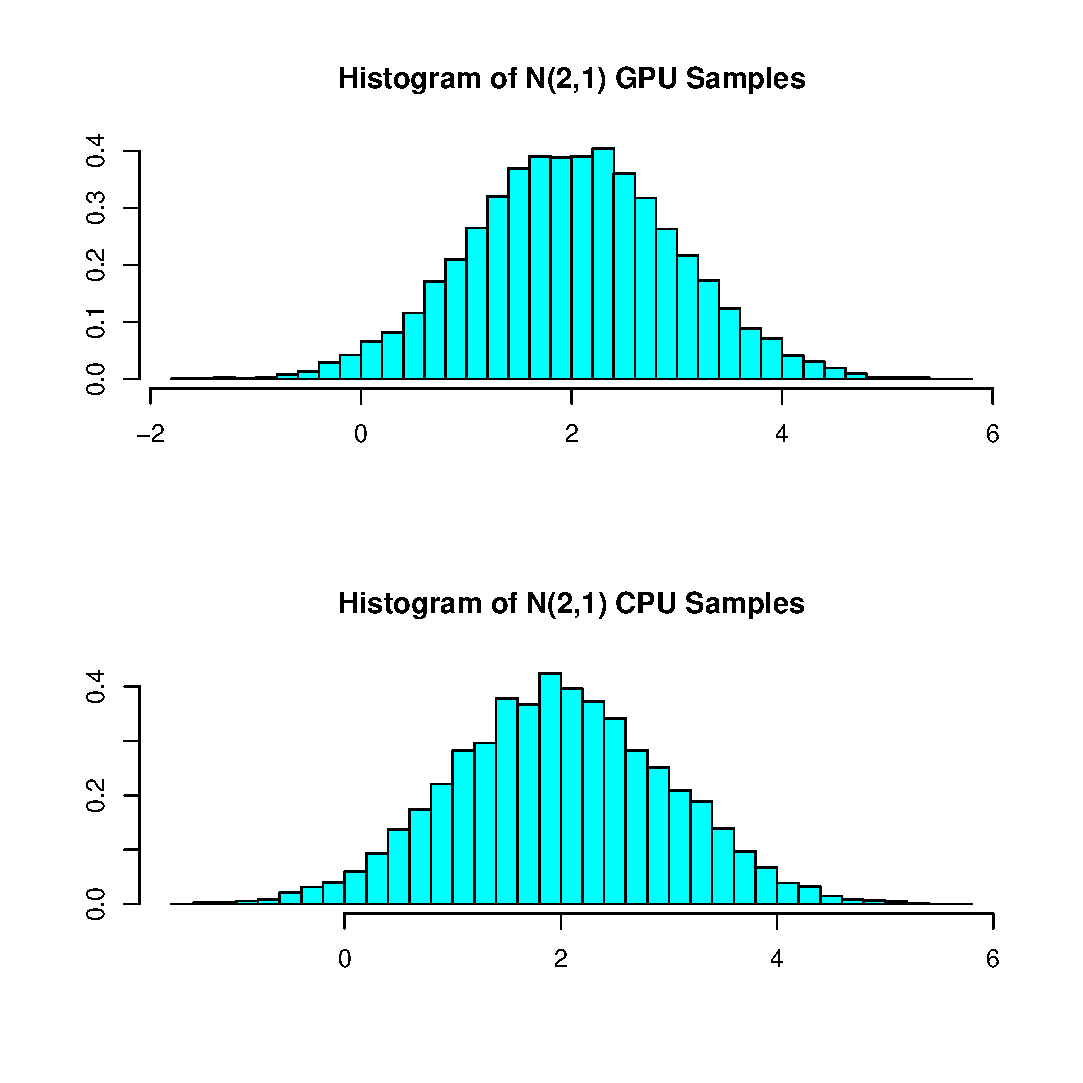
\includegraphics[scale=.45]{TruncNorm/No_TruncNorm_Hist}
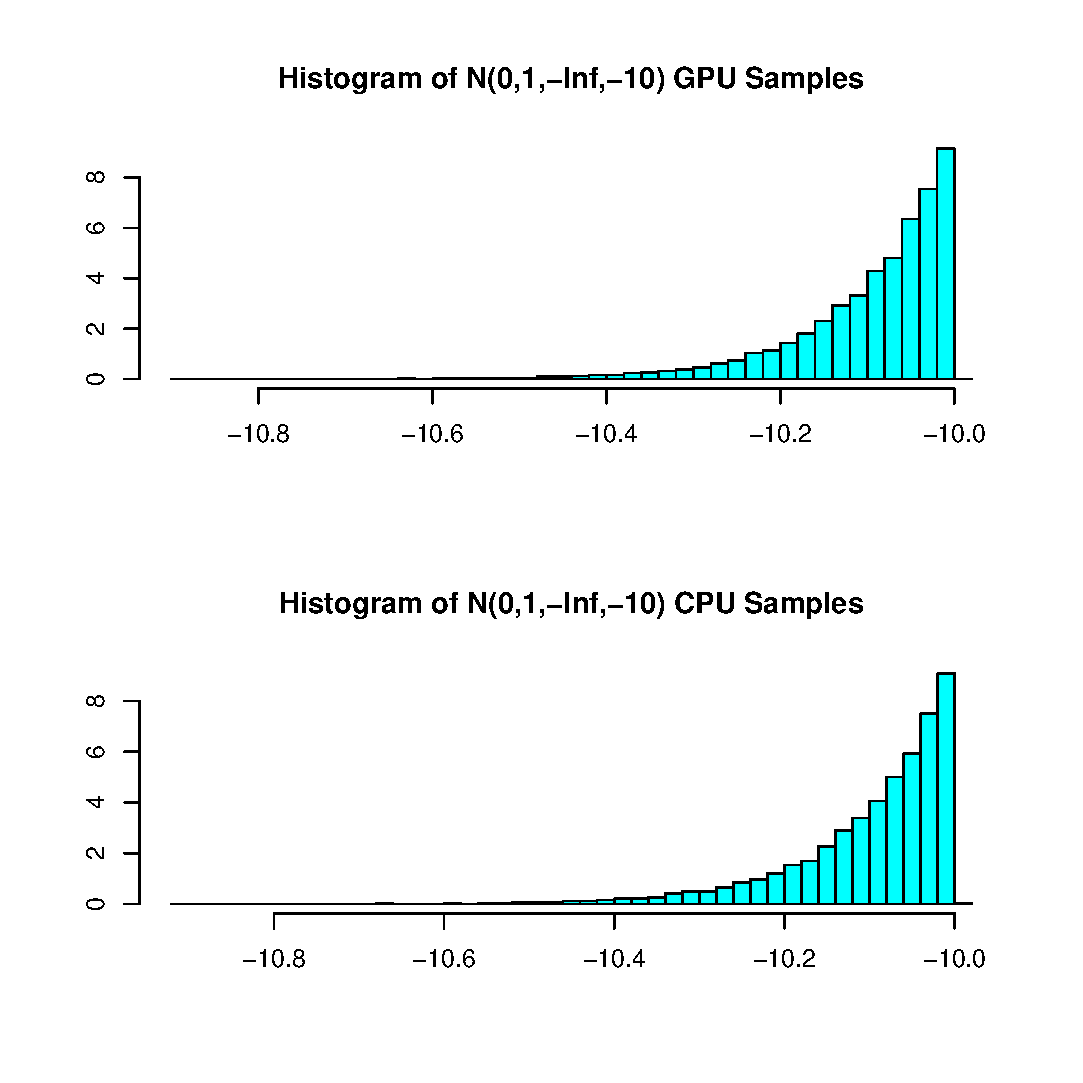
\includegraphics[scale=.45]{TruncNorm/Tail_TruncNorm_Hist}
\end{figure}

\section{Bayesian Probit Regression}
Now that we have a (somewhat) working truncated normal sampler, let's direct our attention to an actual problem: Bayesian probit regression. The idea is simple: We observe an indicator function $y$ of an unobserved latent variable, $z$. To assess a relationship between $y$ and some covariates, we suppose that our $z$'s have a linear relationship to the covariates. If we impose normality on the latent variables, we can say that the probability of $y=1$ is $p = \Phi(X^T \beta)$. Probit regression is not a huge leap of the imagination if one is familiar with logistic regression--the difference is simply the choice of the link function. The goal is to estimate the influence of the covariates $\beta$ on the probability of observed $y$ being 1 or 0. Being Bayesians, we can also place prior belief on the values for $\beta$.

For this analysis, we place a completely diffuse, conditionally conjugate prior on $\beta$. Let $n$ denote the sample size and $p$ denote the number of covariates (including intercept).
\begin{align*}
& \beta \sim N(\beta_0=0_p, \Sigma_0^{-1} = 0_{p \times p}) \\
& z_i | \beta \sim N(X^T \beta_i, 1) \\
& y_i | z_i = 1_{(z_i > 0)}
\end{align*}

We sample from the posterior of $\beta$, given $y$, using Gibbs Sampling.
\begin{align*}
& z_i^t | \beta^t, y_i=0 \sim N(X^T \beta_i^t, 1) 1_{(-\infty, 0)} \\
& z_i^t | \beta^t, y_i=1 \sim N(X^T \beta_i^t, 1) 1_{(0, \infty)} \\
& \beta^{t+1} | z^t, y \sim N(b_z, \Sigma),
\end{align*}
where the posterior variance $\Sigma$ is a combination of the prior variance and the variance of the OLS estimator,
\[ \Sigma = (\Sigma_0^{-1} + X'X)^{-1}, \]
and the posterior mean is similar to the OLS estimate with an additional term to account for prior mean,
\[ b_z = \Sigma (\Sigma_0^{-1} \beta_0 + X'z ) \]

It is worth noticing that at each step, with a completely diffuse prior as we have, the posterior mean and variance are identical to the distribution of the classical least squares estimate if we regressed $z$ on our covariates. Our algorithm for getting posterior samples will thus be:
\begin{enumerate}[A]
\item Set $\beta^1 = (X'X)^{-1} X'y$, the least squares solution.
\item Determine truncation points: $L_i = -\infty 1_{y_i = 0}$, $H_i = \infty 1_{y_i = 1}$, for $i=1, \dots, n$.
\end{enumerate}

For each $i = 1, \dots,$ maxiter:
\begin{enumerate}
\item Sample $z_i$ from $TN(X' \beta^i, 1, (L_i, H_i))$
\item Sample $\beta^{t+1}$ from Multivariate $N(b_z, \Sigma)$. 
\end{enumerate}

A faux-CUDA version is implemented by swapping out the truncated normal sampler for a GPU-version. Ideally, a GPU implementation would do the multivariate normal, the truncated normal, and possibly some of the matrix math on the GPU. This proved unwieldy for memory management reasons. A more intelligent method of manipulating memory might alleviate some of this strain. Not having to transfer the latent variable $z$'s off the GPU could drastically improve performance.

Testing the CPU and GPU implementations on $n=1000$ dataset, the posterior matches up nicely with the true underlying values of $\beta$. Setting the initial value at the OLS estimator was smart--technically, we did not need a 500-sample burn-in, and burning 500 observations didn't do much for us. 

What did kill us, however, was the number of iterations. Having to pass around the latent variables device the device and host was devastating for a larger data set. The actual computation was inconsequential in comparison. If I had managed my own memory, I wouldn't have passed the latent variables back and forth between device and host. Ideally, level 2 BLAS functionality could've done the math on the GPU itself, as the only time I needed the latent variables was in calculating the posterior mean of $\beta$.

\begin{figure}[H] \center
\includegraphics[scale=.45]{Probit/Probit_Timings}
\end{figure}

The serial implementation increased in runtime linearly with the sample size. From my pure-C implementation of the truncated normal when I was developing it, I noticed the computing time was relatively constant, or at least scaled far better than the computing time of the CPU implementation. There is no runtime available for the final dataset on the GPU--it took too long to run.

If the memory copies and allocation could be done once and written over when needed, I am certain the GPU would beat the CPU implementation after the initial cost of allocating memory on the GPU took the same amount of time as computing samples on the CPU. This is problem-dependent, but it is possible we could see a significant speedup as soon as a sample size of 100,000 or 1,000,000.

\newpage
\section*{R Source Code}
The CUDA truncated normal kernel and helper functions.
\lstinputlisting[language=C++]{"k_tnorm.cu"}

\newpage

Functions to run the make file, load the CUDA kernel into R, and make it interface nicer with R.
\lstinputlisting{"helper_functions.R"}

Code to put the truncated normal sampler through its paces:
\lstinputlisting{"TruncNorm/TruncNorm.R"}

Code to do Bayesian probit regression:
\lstinputlisting{"Probit/probit_mcmc.R"}
\end{document} 